% Provenance (never printed): see sources/outline_sources.md (Year 2: radiogenic tracers
% Sr, Nd, Pb and mantle reservoirs; crustal growth; stable isotopes, delta notation and
% fractionation, d18O and d13C). Curves from figdata/bachelor-2/isotopes.py; exercise and
% problem values in the Book 4 scratch calculators calc/ch04.py and calc/ch04pb.py.
% Ruling (Sync 2): delta value and fractionation factor are chemistry's (Year 3 volume),
% recalled; this chapter defines the reference standards and the meteoric water line.
\chapter{Geoquímica isotópica}\label{ch:b2:isotope-geochemistry}

Mangaia, en el Pacífico sur, y Tristán de Acuña, en el Atlántico
sur, son dos islas volcánicas de basalto, y una muestra de mano de
una se parece mucho a una muestra de mano de la otra, o de una dorsal oceánica.
Sus isótopos las distinguen. El estroncio de los basaltos de Mangaia lleva
la misma proporción de estroncio-87 que el de las dorsales, cerca de
$^{87}\mathrm{Sr}/^{86}\mathrm{Sr} = 0.7028$, mientras que su plomo está entre los más
radiogénicos de la Tierra, con $^{206}\mathrm{Pb}/^{204}\mathrm{Pb}$ cerca de 21.6 frente a
18.4 en las dorsales. Los basaltos de Tristán contienen más estroncio-87, de 0.7050 a
0.7054, y menos neodimio-143 que ambos. La fusión no separa los isótopos de
estos elementos pesados, de modo que cada lava lleva la firma isotópica del
manto que se fundió para formarla: el manto terrestre no es un reservorio sino
varios, que han conservado razones padre--hijo distintas durante miles de millones de
años. Este capítulo usa la desintegración radiactiva del rubidio, el samario, el uranio
y el torio como un conjunto de trazadores, sigue la evolución del manto y de la
corteza continental a través de los isótopos del neodimio, separa el manto en
reservorios y mezclas de reservorios, discute con qué rapidez crecieron los continentes,
y termina con los isótopos estables ligeros del oxígeno, el hidrógeno y el carbono, que
trazan el agua y el carbono a través de la Tierra.
% ledger: data:b4-oib-isotopes, gale13:isotopes

\begin{recall}
Un padre radiactivo se desintegra al ritmo $\lambda P$, y en un sistema cerrado la
razón del hijo crece como $(D/D_s)_{\text{actual}} = (D/D_s)_0 + (P/D_s)_{\text{actual}}
(e^{\lambda t}-1)$, siendo $D_s$ un isótopo estable del hijo; los minerales o
rocas formados a la vez se sitúan sobre una isócrona, cuya pendiente da la edad y cuya
ordenada en el origen da la razón inicial (volumen de bachillerato, último año; volumen de primer año,
capítulo sobre la datación radiométrica). Un espectrómetro de masas separa los iones por su
relación masa/carga (volumen de segundo año de los libros de química). El valor $\delta$ de una
muestra es $\delta = (R_{\text{muestra}}/R_{\text{patrón}} - 1)\times 1000$, en tanto
por mil, y el factor de fraccionamiento entre dos fases A y B es
$\alpha_{\mathrm{A/B}} = R_{\mathrm A}/R_{\mathrm B}$, siendo $R$ la razón del
isótopo pesado al ligero; ambos se presentan, con las energías de punto cero
que causan el fraccionamiento isotópico, en el volumen de tercer año de los libros de química.
Los \omterm{def:b2:elements-in-the-earth:partition}{elementos incompatibles}, el MORB y el OIB se definieron en el
\cref{ch:b2:elements-in-the-earth}.
\end{recall}

\section{Los isótopos radiogénicos como trazadores}

Tres sistemas de desintegración llevan la mayor parte de la información sobre el manto y la corteza.
El rubidio-87 se desintegra en estroncio-87, el samario-147 en neodimio-143, y el uranio
y el torio, a través de sus cadenas de desintegración, en tres isótopos del plomo. Cada padre
y su hijo difieren en su comportamiento durante la fusión, y cada hijo tiene un
isótopo estable, no radiogénico, frente al que se mide.

\begin{table}[ht]
\centering
\begin{tabular}{lllll}
\hline
padre & hijo & razón medida & constante de desintegración (por año) & semivida (Ga)\\
\hline
$^{87}$Rb & $^{87}$Sr & $^{87}\mathrm{Sr}/^{86}\mathrm{Sr}$ & \num{1.3972e-11} & 49.6\\
$^{147}$Sm & $^{143}$Nd & $^{143}\mathrm{Nd}/^{144}\mathrm{Nd}$ & \num{6.524e-12} & 106.25\\
$^{238}$U & $^{206}$Pb & $^{206}\mathrm{Pb}/^{204}\mathrm{Pb}$ & \num{1.55125e-10} & 4.47\\
\hline
\end{tabular}
\caption{Tres sistemas de desintegración de vida larga usados como trazadores. Datos: recomendaciones
IUPAC--IUGS (Villa y colaboradores, 2020 y 2022).}
\label{tab:b2:isotope-geochemistry:decay}
\end{table}
% ledger: villa22:rb87, villa20:sm147

\begin{definition}[Trazador isotópico radiogénico]\label{def:b2:isotope-geochemistry:tracer}
Un \emph{trazador isotópico radiogénico}\index{trazador isotópico radiogénico} es la razón
entre un isótopo hijo producido por un padre radiactivo de vida larga y un isótopo
estable del mismo elemento, como $^{87}\mathrm{Sr}/^{86}\mathrm{Sr}$ o
$^{143}\mathrm{Nd}/^{144}\mathrm{Nd}$, que se usa para identificar la fuente de una roca más que
para datarla. La razón de un reservorio crece a un ritmo fijado por su
razón padre--hijo, y registra así la historia de esa razón.
\end{definition}

Los dos elementos de un par de desintegración se separan siempre que el manto se funde. En el
\cref{ch:b2:elements-in-the-earth}, el rubidio resultó más incompatible que el
estroncio y el neodimio más incompatible que el samario. Un fundido, y la corteza
que construye, abandonan por tanto el manto con una Rb/Sr alta y una Sm/Nd baja; el
residuo conserva una Rb/Sr baja y una Sm/Nd alta. Con el tiempo la corteza gana
estroncio-87 más deprisa que su fuente y neodimio-143 más despacio; el \omterm{def:b2:isotope-geochemistry:reservoirs}{manto
empobrecido} hace lo contrario. Las razones de los dos pares se mueven en sentidos
opuestos, algo que el diagrama Sr--Nd siguiente pone de manifiesto.

\begin{proposition}[Las razones isotópicas sobreviven a la fusión]\label{prop:b2:isotope-geochemistry:melting}
Cuando una roca se funde y el fundido se separa del residuo, las razones
$^{87}\mathrm{Sr}/^{86}\mathrm{Sr}$ y $^{143}\mathrm{Nd}/^{144}\mathrm{Nd}$ del
fundido son iguales a las de la fuente dentro de la precisión de las
medidas; solo cambian las razones padre--hijo, Rb/Sr y Sm/Nd.
\end{proposition}
\admitted

\noindent El enunciado descansa en dos hechos. Los isótopos de un elemento tienen la
misma estructura electrónica, de modo que entran en un cristal o en un fundido casi por igual; la
diferencia relativa de masa entre el estroncio-87 y el estroncio-86, cerca de un uno por
ciento, es mucho menor que en el oxígeno o el hidrógeno, y a alta temperatura el
logaritmo de un factor de fraccionamiento de equilibrio decrece como el inverso del cuadrado de
la temperatura, hacia 1. Y la propia medida corrige el
fraccionamiento que se produce en el espectrómetro de masas fijando una razón de dos
isótopos no radiogénicos (para el neodimio, $^{146}\mathrm{Nd}/^{144}\mathrm{Nd} =
0.7219$), lo que borraría también cualquier pequeño fraccionamiento natural. Una lava,
por tanto, muestrea las razones isotópicas de su fuente, mientras que sus razones de
\omterm{def:b2:elements-in-the-earth:trace}{elementos en trazas} reflejan también la fusión.
% ledger: white:chur, white:t-dependence

\section{La evolución del manto y de la corteza}

\subsection{El reservorio condrítico}

El samario y el neodimio son ambos \omterm{def:b2:elements-in-the-earth:ree}{tierras raras} litófilas refractarias
(\cref{ch:b2:elements-in-the-earth}): la \omterm{def:b2:elements-in-the-earth:bse}{Tierra silicatada global} debería haber conservado
su razón condrítica. Las \omterm{def:b2:planet-formation-meteorites:chondrule}{condritas} dan entonces la historia Sm--Nd de la
Tierra no diferenciada.

\begin{definition}[Reservorio condrítico uniforme]\label{def:b2:isotope-geochemistry:chur}
El \emph{reservorio condrítico uniforme}\index{reservorio condrítico uniforme}
(CHUR) es un reservorio modelo con la composición en samario--neodimio de las
\omterm{def:b2:planet-formation-meteorites:chondrule}{condritas}, cerrado desde la formación del sistema solar. Sus razones
actuales son $(^{143}\mathrm{Nd}/^{144}\mathrm{Nd})_{\mathrm{CHUR}} = 0.512638$ y
$(^{147}\mathrm{Sm}/^{144}\mathrm{Nd})_{\mathrm{CHUR}} = 0.1966$.
\end{definition}
% ledger: white:chur

Remontando el tiempo con la ecuación de la isócrona, el CHUR tenía, cuando condensaron los primeros
sólidos hace \qty{4567}{Myr} (\cref{ch:b2:planet-formation-meteorites}),
\[
  ^{143}\mathrm{Nd}/^{144}\mathrm{Nd} = 0.512638 - 0.1966\,\bigl(e^{\lambda\cdot
  \num{4.567e9}\,\mathrm{yr}}-1\bigr) = 0.506692 .
\] Desde entonces su razón ha crecido un
1.2 por ciento. Las diferencias entre las rocas terrestres son mil veces
menores, y se expresan en una unidad más cómoda.
% ledger: lugaro:cai, villa20:sm147

\begin{definition}[Notación épsilon]\label{def:b2:isotope-geochemistry:epsilon}
La \emph{notación épsilon}\index{notación épsilon} expresa la razón
$^{143}\mathrm{Nd}/^{144}\mathrm{Nd}$ de una muestra, en un tiempo $t$ antes del
presente, como su desviación relativa respecto al CHUR en el mismo tiempo, en partes por diez
mil:
\[
  \varepsilon_{\mathrm{Nd}}(t) = \left(
  \frac{(^{143}\mathrm{Nd}/^{144}\mathrm{Nd})_{\text{muestra}}(t)}
       {(^{143}\mathrm{Nd}/^{144}\mathrm{Nd})_{\mathrm{CHUR}}(t)} - 1\right)\times 10^4 .
\]
Sin tiempo, $\varepsilon_{\mathrm{Nd}}$ es el valor actual.
\end{definition}

El MORB medio, con $^{143}\mathrm{Nd}/^{144}\mathrm{Nd} = 0.513074$, tiene
$\varepsilon_{\mathrm{Nd}} = (0.513074/0.512638 - 1)\times10^4 = +8.5$; la mayoría de las rocas
están entre $-20$ y $+10$. Un valor positivo significa que la fuente de la roca
ha tenido, en promedio a lo largo de la historia de la Tierra, una Sm/Nd más alta que las
\omterm{def:b2:planet-formation-meteorites:chondrule}{condritas}: está empobrecida en el elemento más incompatible, el neodimio. Un
valor negativo significa lo contrario. El alejamiento de la Sm/Nd condrítica se mide por la
desviación fraccional
\[
  f_{\mathrm{Sm/Nd}} = \frac{(\mathrm{Sm}/\mathrm{Nd})_{\text{muestra}}}
  {(\mathrm{Sm}/\mathrm{Nd})_{\mathrm{CHUR}}} - 1,
\]
que es la misma tanto si las razones son másicas como atómicas. Con los valores CI
del \cref{ch:b2:elements-in-the-earth} (Sm 0.145, Nd \qty{0.457}{ppm},
$\mathrm{Sm}/\mathrm{Nd} = 0.317$), la corteza continental superior (4.7 y
\qty{27}{ppm}, 0.174) tiene $f_{\mathrm{Sm/Nd}} = -0.45$.
% ledger: gale13:isotopes, white:chur, lodders:ci-table, rg03:ucc-trace

\begin{proposition}[Crecimiento lineal de $\varepsilon_{\mathrm{Nd}}$]\label{prop:b2:isotope-geochemistry:linear}
Un reservorio que se separó del CHUR y ha conservado desde entonces la desviación fraccional
$f_{\mathrm{Sm/Nd}}$ cambia su $\varepsilon_{\mathrm{Nd}}$, hacia adelante en el
tiempo, al ritmo
\[
  \frac{\mathrm{d}\varepsilon_{\mathrm{Nd}}}{\mathrm{d}\tau} \approx Q\,f_{\mathrm{Sm/Nd}},
  \qquad
  Q = 10^4\,\lambda_{147}\,
  \frac{(^{147}\mathrm{Sm}/^{144}\mathrm{Nd})_{\mathrm{CHUR}}}
       {(^{143}\mathrm{Nd}/^{144}\mathrm{Nd})_{\mathrm{CHUR}}}
  = \qty{25.0}{\per\giga\year},
\]
donde $\tau$ es el tiempo contado hacia adelante. Un reservorio con $\varepsilon_0$ en su
separación, hace un tiempo $T$, tiene hoy $\varepsilon_{\mathrm{Nd}} \approx \varepsilon_0
+ Q f_{\mathrm{Sm/Nd}} T$.
\end{proposition}

\begin{proof}
Escríbase $R$ por $^{143}\mathrm{Nd}/^{144}\mathrm{Nd}$ y $p$ por
$^{147}\mathrm{Sm}/^{144}\mathrm{Nd}$. En un reservorio cerrado
$\mathrm{d}R/\mathrm{d}\tau = \lambda p\,e^{\lambda t}$, con $t$ el tiempo antes del
presente; como $\lambda t \le 0.03$, el factor $e^{\lambda t}$ difiere de 1 como
mucho en un 3 por ciento, y $\mathrm{d}R/\mathrm{d}\tau \approx \lambda p$. Entonces
$\mathrm{d}(R_s - R_c)/\mathrm{d}\tau \approx \lambda (p_s - p_c) = \lambda p_c
f_{\mathrm{Sm/Nd}}$, ya que $p_s/p_c - 1 = f_{\mathrm{Sm/Nd}}$. Dividiendo por $R_c$,
que solo cambia un 1.2 por ciento a lo largo de la edad de la Tierra, se obtiene
$\mathrm{d}\varepsilon/\mathrm{d}\tau \approx 10^4\lambda p_c f/R_c$. Con
$\lambda = \qty{6.524e-12}{\per\year}$, $p_c = 0.1966$ y $R_c = 0.512638$, $Q =
\num{2.502e-8}$ por año, \qty{25.0}{\per\giga\year}.
\end{proof}
% ledger: villa20:sm147, white:chur

Una corteza con la Sm/Nd de la corteza superior ($f = -0.45$) pierde por tanto unas
11 unidades épsilon por cada mil millones de años respecto al CHUR, mientras que a un reservorio del manto
le basta $f = +0.07$ para subir de 0 al valor del MORB, $+8.5$, en
\qty{4.567}{Ga}. La figura siguiente sigue las ecuaciones exactas de tres
reservorios: el CHUR, un \omterm{def:b2:isotope-geochemistry:reservoirs}{manto empobrecido} cerrado desde la formación de la Tierra con la Sm/Nd
que lo lleva hoy al valor del MORB ($^{147}\mathrm{Sm}/^{144}\mathrm{Nd} =
0.211$), y una corteza extraída de ese manto hace 2700 millones de años con la
Sm/Nd de la corteza superior ($0.108$). La corteza partió de $\varepsilon_{\mathrm{Nd}} =
+3.5$, el valor de su fuente en ese momento, y hoy está en $-27$.

\begin{definition}[Manto empobrecido, manto enriquecido]\label{def:b2:isotope-geochemistry:reservoirs}
Un \emph{manto empobrecido}\index{manto empobrecido} es una parte del manto que ha
perdido \omterm{def:b2:elements-in-the-earth:partition}{elementos incompatibles} en favor de fundidos, de modo que su Sm/Nd es más alta y su Rb/Sr
más baja que las condríticas; con el tiempo su $\varepsilon_{\mathrm{Nd}}$ se vuelve positiva y
su $^{87}\mathrm{Sr}/^{86}\mathrm{Sr}$ baja. Un \emph{manto
enriquecido}\index{manto enriquecido} es una parte del manto que ha ganado
\omterm{def:b2:elements-in-the-earth:partition}{elementos incompatibles}, por ejemplo de corteza reciclada o de fundidos pequeños,
con una $\varepsilon_{\mathrm{Nd}}$ negativa o una $^{87}\mathrm{Sr}/^{86}\mathrm{Sr}$ alta.
\end{definition}

\begin{omfigure}
\centering
\begin{tikzpicture}
\begin{axis}[omrecord, width=0.82\linewidth, height=6.4cm,
  x dir=reverse, xmin=0, xmax=4.6, ymin=-30, ymax=12,
  xlabel={tiempo antes del presente (Ga)}, ylabel={$\varepsilon_{\mathrm{Nd}}(t)$},
  tick label style={font=\scriptsize}, label style={font=\small}]
\addplot[thick, black] table[x=t_Ga, y=eps] {figdata/out/bachelor-2-isotopes-chur.dat};
\addplot[very thick, blue!70!black] table[x=t_Ga, y=eps] {figdata/out/bachelor-2-isotopes-dm.dat};
\addplot[very thick, brown!70!black] table[x=t_Ga, y=eps] {figdata/out/bachelor-2-isotopes-crust.dat};
\addplot[densely dashed, gray] coordinates {(2.7,-30) (2.7,12)};
\node[font=\scriptsize, anchor=north] at (axis cs:3.6,-0.6) {CHUR};
\node[font=\scriptsize, blue!70!black, anchor=south east] at (axis cs:0.4,8.8) {manto empobrecido, $+8.5$};
\node[font=\scriptsize, brown!70!black, anchor=north east] at (axis cs:0.3,-25.5) {corteza, $-27$};
\node[font=\scriptsize, gray, anchor=north west, align=left] at (axis cs:2.65,-12) {corteza extraída\\a \qty{2.7}{Ga}};
\end{axis}
\end{tikzpicture}
\par\smallskip{\small Evolución isotópica del neodimio, como $\varepsilon_{\mathrm{Nd}}$, del
reservorio condrítico (cero por definición), de un \omterm{def:b2:isotope-geochemistry:reservoirs}{manto empobrecido} cerrado desde
\qty{4.567}{Ga} cuya Sm/Nd lo lleva hoy al MORB medio, y de una corteza
extraída de él hace \qty{2.7}{Ga} con la Sm/Nd de la corteza continental
superior. Cada línea es casi recta, como dice la proposición del crecimiento lineal. Datos:
CHUR, el manual de White; MORB medio, Gale y colaboradores (2013); Sm/Nd de la corteza,
Rudnick y Gao.}
\end{omfigure}
% ledger: white:chur, villa20:sm147, gale13:isotopes, rg03:ucc-trace, lodders:ci-table, lugaro:cai

\subsection{Dos reservorios complementarios}

Si la corteza continental y el \omterm{def:b2:isotope-geochemistry:reservoirs}{manto empobrecido} se formaron a partir de un solo reservorio
condrítico, su neodimio debe sumar de nuevo el valor condrítico. El neodimio es
el portador: cada reservorio cuenta en proporción al neodimio que contiene.

\begin{proposition}[Balance de masas isotópico]\label{prop:b2:isotope-geochemistry:mass-balance}
Sean reservorios $i$ de masas $M_i$ y concentraciones de neodimio $C_i$ procedentes de
la división de un reservorio padre. Entonces, con muy buena aproximación,
\[
  \sum_i M_i C_i\, \varepsilon_i = \Bigl(\sum_i M_i C_i\Bigr) \varepsilon_{\text{padre}},
\]
evaluándose ambos miembros en el mismo tiempo, y siguiéndose al padre como si
hubiera permanecido entero.
\end{proposition}

\begin{proof}
El número de átomos de $^{143}\mathrm{Nd}$ y el número de átomos de $^{144}\mathrm{Nd}$
se conservan cada uno en la división, y después cada uno crece (en el caso del
$^{143}\mathrm{Nd}$) o permanece (en el del $^{144}\mathrm{Nd}$) en cada reservorio exactamente como
en el conjunto. Por tanto la media ponderada por el $^{144}\mathrm{Nd}$ de las razones $R_i$ es igual a
la razón del padre, $R_p$. La proporción de $^{144}\mathrm{Nd}$ en el neodimio varía
entre reservorios mucho menos de una parte por mil, de modo que ponderar por
$M_iC_i$ equivale a ponderar por el $^{144}\mathrm{Nd}$. Por último, $\varepsilon$ es una
función lineal de $R$ en un tiempo dado, $\varepsilon = 10^4(R/R_c - 1)$, y una
media ponderada de funciones lineales es la función lineal de la media ponderada.
\end{proof}

Si se toma el valor de la corteza superior, \qty{27}{ppm} de neodimio, para toda la
corteza, una corteza continental de \qty{7.2e9}{km^3} a \qty{2830}{kg/m^3}, es decir
\qty{2.0e22}{kg} o el 0.51 por ciento de la masa de la Tierra silicatada, contiene
$0.0051\times27/1.25 = 11$ por ciento del neodimio de la Tierra silicatada (\omterm{def:b2:elements-in-the-earth:bse}{manto
primitivo}, \qty{1.25}{ppm}). Si la corteza tiene una $\varepsilon_{\mathrm{Nd}}$ media de
$-15$, el manto debe compensar una contribución negativa de $0.11\times15 = 1.65$
unidades: un reservorio con el valor del MORB, $+8.5$, tendría que contener
cerca de una quinta parte del neodimio de la Tierra silicatada (\cref{exo:b2:isotope-geochemistry:9}). Es uno de los
argumentos de que el \omterm{def:b2:isotope-geochemistry:reservoirs}{manto empobrecido} que muestrean las dorsales no es todo el
manto.
% ledger: cogley84:continents, cm95:crust, ms95:pm-trace, rg03:ucc-trace, data:prem, earth:mass, gale13:isotopes

\section{Los reservorios del manto}

Las razones isotópicas de los basaltos oceánicos muestrean el manto sin pasar por
la corteza continental. Representadas unas frente a otras, muestran a la vez la
complementariedad entre la corteza y el \omterm{def:b2:isotope-geochemistry:reservoirs}{manto empobrecido} y la existencia de otros
reservorios.

Los isótopos del estroncio y del neodimio están anticorrelacionados en la mayoría de los basaltos oceánicos: una
lava con una $\varepsilon_{\mathrm{Nd}}$ alta tiene una
$^{87}\mathrm{Sr}/^{86}\mathrm{Sr}$ baja. Esta banda se llama la alineación del manto; se debe
al comportamiento opuesto de los dos pares durante la fusión (el rubidio, menos
compatible que el estroncio; el samario, más compatible que el neodimio). El MORB
medio está en su extremo empobrecido, con $^{87}\mathrm{Sr}/^{86}\mathrm{Sr} = 0.702819$ y
$\varepsilon_{\mathrm{Nd}} = +8.5$. Los \omterm{def:b2:elements-in-the-earth:morb-oib}{basaltos de isla oceánica} se extienden desde allí hacia
$\varepsilon_{\mathrm{Nd}}$ más bajas y $^{87}\mathrm{Sr}/^{86}\mathrm{Sr}$ más altas, pero no
a lo largo de una sola línea.
% ledger: white:dm, gale13:isotopes

\begin{definition}[Miembro extremo del manto]\label{def:b2:isotope-geochemistry:end-members}
Un \emph{miembro extremo del manto}\index{miembro extremo del manto} es una de las composiciones
isotópicas extremas a partir de cuya mezcla pueden construirse las razones isotópicas de Sr, Nd y Pb de los
basaltos oceánicos. Se nombran por lo común cuatro: DMM, el \omterm{def:b2:isotope-geochemistry:reservoirs}{manto
empobrecido} de los MORB ($^{87}\mathrm{Sr}/^{86}\mathrm{Sr}$ baja, $\varepsilon_{\mathrm{Nd}}$ alta);
HIMU, por una $\mu = {}^{238}\mathrm{U}/^{204}\mathrm{Pb}$ alta en su fuente
(plomo muy radiogénico, $^{206}\mathrm{Pb}/^{204}\mathrm{Pb}$ por encima de 20, con
$^{87}\mathrm{Sr}/^{86}\mathrm{Sr}$ baja); EM1, el \omterm{def:b2:isotope-geochemistry:reservoirs}{manto enriquecido} 1 (con
$^{87}\mathrm{Sr}/^{86}\mathrm{Sr}$ moderadamente alta, $\varepsilon_{\mathrm{Nd}}$ negativa y plomo
poco radiogénico); y EM2, el \omterm{def:b2:isotope-geochemistry:reservoirs}{manto enriquecido} 2 ($^{87}\mathrm{Sr}/^{86}\mathrm{Sr}$ alta).
\end{definition}
% ledger: white:end-members

\begin{omfigure}
\centering
\begin{tikzpicture}
\begin{axis}[omrecord, width=0.82\linewidth, height=6.6cm,
  xmin=0.7020, xmax=0.7064, ymin=-6, ymax=11,
  xlabel={$^{87}\mathrm{Sr}/^{86}\mathrm{Sr}$}, ylabel={$\varepsilon_{\mathrm{Nd}}$},
  xticklabel style={/pgf/number format/fixed, /pgf/number format/precision=4},
  scaled x ticks=false, legend pos=south west, legend cell align=left,
  legend style={font=\scriptsize}, tick label style={font=\scriptsize},
  label style={font=\small}]
\addplot[only marks, mark=*, mark size=1.3pt, red!70!black] table[x=sr, y=eps] {figdata/out/bachelor-2-isotopes-himu.dat};
\addlegendentry{tipo HIMU: Santa Elena, Mangaia, Tubuai}
\addplot[only marks, mark=square*, mark size=1.2pt, brown!70!black] table[x=sr, y=eps] {figdata/out/bachelor-2-isotopes-em1.dat};
\addlegendentry{tipo EM1: Tristán de Acuña, Gough}
\addplot[only marks, mark=diamond*, mark size=3pt, blue!70!black] table[x=sr, y=eps] {figdata/out/bachelor-2-isotopes-morb.dat};
\addlegendentry{MORB medio}
\addplot[densely dashed, gray] coordinates {(0.7020,0) (0.7064,0)};
\node[font=\scriptsize, gray, anchor=south east] at (axis cs:0.7063,0.1) {CHUR};
\draw[->, gray] (axis cs:0.7030,9.5) -- (axis cs:0.7046,0.8);
\node[font=\scriptsize, gray, anchor=west, align=left] at (axis cs:0.7036,6.5) {la alineación del manto:\\de empobrecido a enriquecido};
\end{axis}
\end{tikzpicture}
\par\smallskip{\small Isótopos del estroncio y del neodimio de 89 basaltos de cinco
islas oceánicas y del basalto medio de dorsal oceánica. Las islas de tipo HIMU se sitúan
por debajo de la alineación principal, con la baja razón del estroncio del MORB pero con una
$\varepsilon_{\mathrm{Nd}}$ más baja; las islas de tipo EM1 están en el lado enriquecido del CHUR.
Las lavas samoanas de tipo EM2 llegan a $^{87}\mathrm{Sr}/^{86}\mathrm{Sr} = 0.7205$, muy
fuera de esta escala, a la derecha. Datos: Stracke y colaboradores (2022), CC BY 4.0; Gale y
colaboradores (2013); Edwards y colaboradores (2019).}
\end{omfigure}
% ledger: data:b4-oib-isotopes, gale13:isotopes, edwards19:samoa, white:chur

Los grupos de islas de la figura anterior no son aleatorios. El grupo de Santa Elena,
que incluye las islas Australes (entre ellas Mangaia y Tubuai) y
Ascensión, se sitúa por debajo de la alineación principal y tiene el plomo más radiogénico
($^{206}\mathrm{Pb}/^{204}\mathrm{Pb}$ por encima de 20; Mangaia llega a 21.5--22.0). El
grupo de Kerguelen, con Tristán de Acuña, Gough y Kerguelen, está a una
$^{87}\mathrm{Sr}/^{86}\mathrm{Sr}$ moderadamente alta y una $\varepsilon_{\mathrm{Nd}}$ negativa, siempre con
plomo poco radiogénico. El grupo de la Sociedad, con Samoa y las Marquesas, define una
tendencia Sr--Nd más tendida que llega a razones de estroncio muy altas: dos lavas samoanas
tienen $^{87}\mathrm{Sr}/^{86}\mathrm{Sr}$ de 0.7186 y 0.7205, más que el agua de mar
actual (0.7092). Los grupos de Santa Elena, de Kerguelen y de la Sociedad son los tipos HIMU,
EM1 y EM2.
% ledger: white:end-members, data:b4-oib-isotopes, edwards19:samoa

Una razón que difiere entre dos partes del manto ha tenido que ser
mantenida por una diferencia de razón padre--hijo durante mucho tiempo: una
diferencia de 10 unidades de $\varepsilon_{\mathrm{Nd}}$ requiere, según la proposición del
crecimiento lineal, mil millones de años con $f = 0.4$ o cuatro mil millones de años con $f = 0.1$. Los
reservorios del manto son por tanto antiguos. Lo que son se lee en las
razones padre--hijo que exigen sus isótopos. HIMU necesita una U/Pb alta y una
Rb/Sr baja durante mucho tiempo, lo que encaja con una corteza oceánica que perdió plomo y rubidio
en los fluidos liberados sobre una zona de subducción y quedó luego almacenada en el manto
durante uno o dos mil millones de años. EM1 y EM2 necesitan una Sm/Nd baja y, en el caso de EM2, una
Rb/Sr alta: la firma de un material derivado de los continentes, como sedimento
reciclado, o de un \omterm{def:b2:isotope-geochemistry:reservoirs}{manto enriquecido} por fundidos pequeños. Estas interpretaciones se
debaten; las medidas no.
% ledger: white:end-members

\begin{omfigure}
\centering
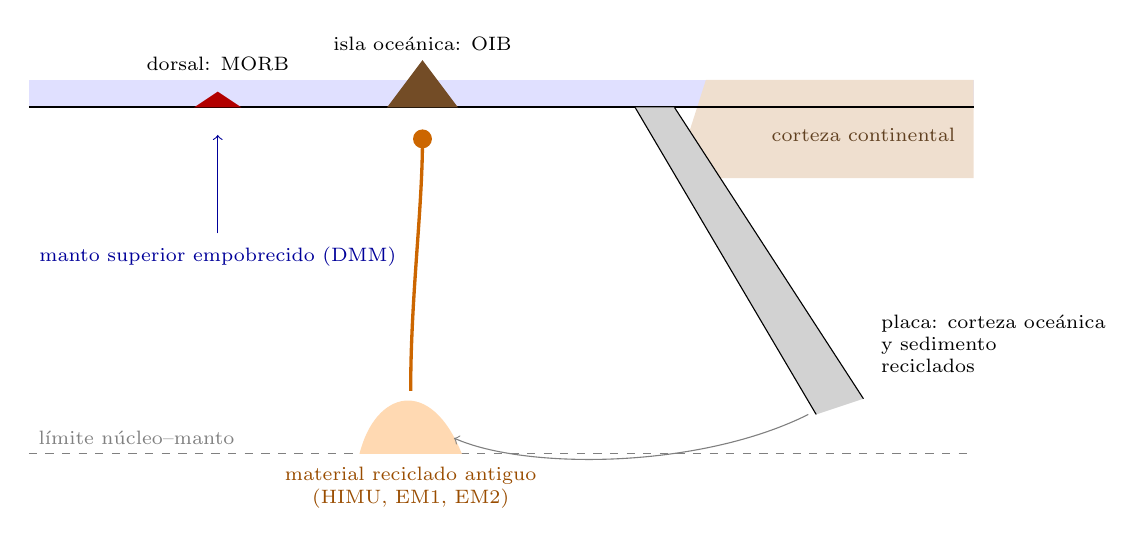
\begin{tikzpicture}[x=1cm, y=1cm, font=\scriptsize]
  % surface and lithosphere
  \fill[blue!12] (-6,0) rectangle (6,0.35);
  \fill[brown!25] (2.6,0.35) -- (6,0.35) -- (6,-0.9) -- (2.2,-0.9) -- cycle;
  \node[brown!50!black] at (4.6,-0.35) {corteza continental};
  \draw[thick] (-6,0) -- (6,0);
  % ridge
  \node[anchor=south] at (-3.6,0.35) {dorsal: MORB};
  \draw[->, blue!60!black] (-3.6,-1.6) -- (-3.6,-0.35);
  \node[blue!60!black, anchor=north] at (-3.6,-1.65) {manto superior empobrecido (DMM)};
  % slab
  \fill[gray!35] (1.7,0) -- (2.2,0) -- (4.6,-3.7) -- (4.0,-3.9) -- cycle;
  \draw (1.7,0) -- (4.0,-3.9) (2.2,0) -- (4.6,-3.7);
  \node[anchor=west, align=left] at (4.7,-3.0) {placa: corteza oceánica\\y sedimento\\reciclados};
  % deep pool and plume
  \draw[gray, dashed] (-6,-4.4) -- (6,-4.4);
  \node[anchor=south west, gray] at (-6,-4.4) {límite núcleo--manto};
  \fill[orange!30] (-1.8,-4.4) .. controls (-1.6,-3.6) and (-0.9,-3.4) .. (-0.5,-4.4) -- cycle;
  \draw[very thick, orange!80!black] (-1.15,-3.6) .. controls (-1.15,-2.4) and (-1.0,-1.3) .. (-1.0,-0.4);
  \fill[orange!80!black] (-1.0,-0.4) circle (0.12);
  \fill[brown!60!black] (-1.45,0) -- (-1.0,0.6) -- (-0.55,0) -- cycle;
  \node[anchor=south] at (-1.0,0.6) {isla oceánica: OIB};
  \fill[red!70!black] (-3.9,0) -- (-3.6,0.2) -- (-3.3,0) -- cycle;
  \node[orange!60!black, anchor=north, align=center] at (-1.15,-4.45) {material reciclado antiguo\\(HIMU, EM1, EM2)};
  \draw[->, gray] (3.9,-3.9) .. controls (2.5,-4.6) and (0.3,-4.6) .. (-0.6,-4.2);
\end{tikzpicture}
\par\smallskip{\small Una interpretación muy extendida de los reservorios del manto, sin
escala: las dorsales muestrean el manto superior empobrecido; la corteza oceánica y el sedimento
vuelven al manto en las zonas de subducción; las plumas que suben del manto profundo
llevan a la superficie material en el que se mezclan componentes reciclados antiguos, y dan a las
islas su carácter HIMU, EM1 o EM2.}
\end{omfigure}

\section{Mezcla}

Muchas alineaciones isotópicas son mezclas. Una lava puede proceder de una fuente que es una
mezcla de dos reservorios, o un magma puede incorporar parte de la corteza que atraviesa.
Los dos casos obedecen a la misma álgebra.

\begin{proposition}[Hipérbola de mezcla]\label{prop:b2:isotope-geochemistry:mixing}
Contenga una mezcla una fracción másica $f$ del componente A y $1-f$ del componente
B. Para un elemento de concentraciones $C_{\mathrm A}$, $C_{\mathrm B}$ y razones
isotópicas $R_{\mathrm A}$, $R_{\mathrm B}$:
\begin{enumerate}
\item la concentración de la mezcla, $C = fC_{\mathrm A} + (1-f)C_{\mathrm B}$, y
su razón isotópica,
$R = \bigl(fC_{\mathrm A}R_{\mathrm A} + (1-f)C_{\mathrm B}R_{\mathrm B}\bigr)/C$, cumplen
$R = a + b/C$ con constantes $a$ y $b$: las mezclas están sobre una recta en
un diagrama de $R$ frente a $1/C$;
\item dos razones de este tipo de dos elementos, $R$ y $R'$, están sobre una hipérbola, llamada
\emph{hipérbola de mezcla}\index{hipérbola de mezcla}, que solo es una recta
si la razón de los dos elementos es la misma en A y en B. Su curvatura la fija
$K = (C'/C)_{\mathrm A}/(C'/C)_{\mathrm B}$.
\end{enumerate}
\end{proposition}

\begin{proof}
(1) Elimínese $f$: $f = (C - C_{\mathrm B})/(C_{\mathrm A} - C_{\mathrm B})$. Entonces
$RC = C_{\mathrm B}R_{\mathrm B} + f(C_{\mathrm A}R_{\mathrm A} - C_{\mathrm B}R_{\mathrm
B})$ es lineal en $C$, $RC = \alpha + \beta C$, y $R = \beta + \alpha/C$.
(2) La proporción del elemento que procede de A es $s = fC_{\mathrm A}/C$, y $R =
R_{\mathrm B} + s(R_{\mathrm A} - R_{\mathrm B})$ es lineal en $s$; del mismo modo $R'$ es
lineal en $s' = fC'_{\mathrm A}/C'$. Con $u = f/(1-f)$, $s = u C_{\mathrm
A}/(uC_{\mathrm A} + C_{\mathrm B})$ y $s' = uC'_{\mathrm A}/(uC'_{\mathrm A} +
C'_{\mathrm B})$. Eliminando $u$ se obtiene $s' = Ks/(1 + (K-1)s)$, una hipérbola en el
plano $(s, s')$, y por tanto en el plano $(R, R')$; es la recta $s' = s$
cuando $K = 1$.
\end{proof}

\begin{omfigure}
\centering
\begin{tikzpicture}
\begin{axis}[omrecord, width=0.62\linewidth, height=6.2cm,
  xmin=0, xmax=1, ymin=0, ymax=1,
  xlabel={primera razón, reescalada (B $=0$, A $=1$)},
  ylabel={segunda razón, reescalada},
  tick label style={font=\scriptsize}, label style={font=\small}]
\addplot[thick, red!70!black] table[x=x, y=y] {figdata/out/bachelor-2-isotopes-mixK50.dat};
\addplot[thick, black] table[x=x, y=y] {figdata/out/bachelor-2-isotopes-mixK10.dat};
\addplot[thick, blue!70!black] table[x=x, y=y] {figdata/out/bachelor-2-isotopes-mixK02.dat};
\node[font=\scriptsize, red!70!black, anchor=south east] at (axis cs:0.30,0.72) {$K=5$};
\node[font=\scriptsize, anchor=south east] at (axis cs:0.55,0.56) {$K=1$};
\node[font=\scriptsize, blue!70!black, anchor=north west] at (axis cs:0.62,0.22) {$K=0.2$};
\node[font=\scriptsize, anchor=north west] at (axis cs:0.0,0.0) {B};
\node[font=\scriptsize, anchor=south east] at (axis cs:1.0,1.0) {A};
\end{axis}
\end{tikzpicture}
\par\smallskip{\small Curvas de mezcla entre dos componentes A y B para tres
valores de $K$, la razón de los dos elementos en A dividida por la de B. Cada
razón isotópica se reescala a 0 en B y a 1 en A; el segundo elemento es $K$ veces
más abundante en A, respecto al primero, que en B, de modo que la segunda razón se acerca a
A más deprisa cuando $K > 1$.}
\end{omfigure}

Un componente rico en un elemento domina la razón isotópica de ese elemento en
la mezcla. Un sedimento reciclado contiene decenas de veces más neodimio que el
\omterm{def:b2:isotope-geochemistry:reservoirs}{manto empobrecido}, y unos pocos por ciento de él en una fuente del manto llevan la
$\varepsilon_{\mathrm{Nd}}$ de la mezcla la mayor parte del camino hacia la suya (problema).
Las islas de tipo HIMU de la figura Sr--Nd quedan fuera de toda curva de mezcla entre el MORB
y las islas EM1: ninguna mezcla de dos componentes explica todos los basaltos oceánicos,
y los miembros extremos son al menos cuatro. Un magma que asimila corteza
continental se desplaza a lo largo de una curva de mezcla hacia la corteza; su posición en la curva
da la proporción de corteza incorporada, un cálculo que se retoma junto con la cristalización
en el \cref{ch:b2:magmatic-differentiation}.

\section{El crecimiento de la corteza continental}

La corteza continental es el complemento del \omterm{def:b2:isotope-geochemistry:reservoirs}{manto empobrecido}; con qué rapidez se
extrajo es una de las cuestiones más antiguas de la geoquímica isotópica, y sigue
abierta. Varios registros aportan datos.

\begin{definition}[Curva de crecimiento cortical]\label{def:b2:isotope-geochemistry:growth}
Una \emph{curva de crecimiento cortical}\index{curva de crecimiento cortical} da el volumen, o
la masa, de corteza continental existente en función del tiempo, como fracción del
volumen actual. Refleja el balance entre la generación de corteza nueva
a partir del manto y su destrucción por reciclaje en el manto.
\end{definition}

Las rocas conservadas hoy dan una primera curva: menos de una cuarta parte del volumen
de la corteza continental juvenil conservada hoy es más antigua que \qty{3}{Ga}, y
ninguna roca conocida tiene una edad de cristalización superior a \qty{4.02}{Ga}. Pero la
corteza conservada es lo que sobrevivió, no lo que se formó. Otras curvas se construyen a partir de
los isótopos del neodimio de las lutitas, que promedian la corteza superior expuesta a la
erosión en el momento de su depósito; de los isótopos del hafnio de los granos de
circón, que registran si el magma que los cristalizó procedía de corteza nueva o
retrabajada; o de los isótopos del argón del cuarzo hidrotermal, que siguen
la desgasificación de la corteza. Varios modelos recientes de este tipo sitúan al menos entre el 60
y el 80 por ciento del volumen actual de corteza continental ya en su lugar hace
\qty{3}{Ga}. Las dos visiones solo pueden conciliarse si se destruyó mucha corteza
temprana: en un modelo de cajas ajustado a ambos registros, se han generado desde la formación de la Tierra de 2.3 a 2.6 veces el
volumen actual de corteza continental,
y de 1.3 a 1.6 veces ese volumen ha vuelto al manto.
% ledger: dhuime18:growth

Las zonas de subducción actuales muestran el reciclaje en acción. El magmatismo de arco añade
unos 2.5 kilómetros cúbicos de corteza nueva al año, 1.5 en los arcos intraoceánicos y
1.0 en los márgenes continentales (2.7 como media a largo plazo), mientras que la subducción
devuelve unos 3.2 kilómetros cúbicos al año; dentro de las incertidumbres, los
continentes no han crecido al menos durante el Fanerozoico. Los isótopos de los \omterm{def:b2:isotope-geochemistry:end-members}{miembros extremos
del manto}, que exigen corteza y sedimento reciclados, son la otra cara de
la misma cuenta.
% ledger: sv09:growth

\section{Isótopos estables}

Los isótopos de los elementos ligeros, hidrógeno, carbono, nitrógeno, oxígeno y
azufre, no se producen por desintegración en cantidades medibles. Se fraccionan
en cambio por procesos físicos, químicos y biológicos, con diferencias relativas de masa
de hasta un factor dos entre el hidrógeno y el deuterio, y sus
variaciones se expresan como valores $\delta$ respecto a patrones acordados.

\begin{definition}[Patrón isotópico de referencia]\label{def:b2:isotope-geochemistry:standards}
Un \emph{patrón isotópico de referencia}\index{patrón isotópico de referencia} es un
material cuya razón isotópica define el cero de una escala $\delta$. En las ciencias de la Tierra
se usan dos. El \emph{VSMOW}\index{VSMOW} (Vienna Standard Mean Ocean
Water) define el $\delta\mathrm{D}$ y el $\delta^{18}\mathrm{O}$ de las aguas, los silicatos y
la mayoría de los demás materiales; sus razones absolutas son $\mathrm{D}/\mathrm{H} =
\num{1.5575e-4}$ y $^{18}\mathrm{O}/^{16}\mathrm{O} = \num{2.0052e-3}$.
El \emph{VPDB}\index{VPDB} (Vienna Pee Dee Belemnite) define el $\delta^{13}\mathrm{C}$
y el $\delta^{18}\mathrm{O}$ de los carbonatos de baja temperatura; sus razones absolutas
son $^{13}\mathrm{C}/^{12}\mathrm{C} = \num{1.1237e-2}$ y
$^{18}\mathrm{O}/^{16}\mathrm{O} = \num{2.0672e-3}$.
\end{definition}
% ledger: kc98:standards

Los nombres recuerdan la historia: el SMOW era un agua oceánica media, y el PDB el
carbonato de una belemnita fósil de la formación Pee Dee; los materiales originales
se agotaron y se sustituyeron por materiales de referencia calibrados respecto a ellos,
distribuidos por el Organismo Internacional de Energía Atómica en Viena y por el NIST.
En la escala \omterm{def:b2:isotope-geochemistry:standards}{VSMOW}, el oxígeno del \omterm{def:b2:isotope-geochemistry:standards}{VPDB} tiene $\delta^{18}\mathrm{O} = +30.9$ por mil
(\cref{exo:b2:isotope-geochemistry:2}): un carbonato marino es ese tanto más pesado que el agua oceánica en la que
creció.
% ledger: kc98:standards

\subsection{El agua}

El agua oceánica está cerca de $\delta^{18}\mathrm{O} = \delta\mathrm{D} = 0$, por la
definición del \omterm{def:b2:isotope-geochemistry:standards}{VSMOW}. La evaporación favorece los isótopos ligeros: en equilibrio
con agua líquida a \qty{20}{\degreeCelsius}, con factores de fraccionamiento de
1.0098 para el oxígeno-18 y 1.084 para el deuterio, el vapor tendría
$\delta^{18}\mathrm{O} = 1000/1.0098 - 1000 = -9.7$ por mil y $\delta\mathrm{D} =
-77$ por mil; el vapor sobre los océanos es aún más ligero, cerca de $-13$ por mil
en $\delta^{18}\mathrm{O}$, porque la evaporación es también un proceso cinético.
A medida que una masa de aire avanza hacia el interior y hacia los polos y se enfría, pierde agua por la lluvia, y
cada lluvia se lleva primero los isótopos pesados; el vapor restante, y la lluvia y
la nieve que siguen, se vuelven cada vez más ligeros. El hielo de Groenlandia tiene típicamente
un $\delta^{18}\mathrm{O}$ de $-30$ a $-35$ por mil, y el hielo antártico llega a $-50$.
% ledger: kc98:alpha, white:d18o

\begin{proposition}[Recta de agua meteórica]\label{prop:b2:isotope-geochemistry:mwl}
La lluvia y la nieve de todo el mundo, y las aguas dulces derivadas de ellas,
están cerca de la \emph{recta de agua meteórica}\index{recta de agua meteórica}
\[
  \delta\mathrm{D} = 8\,\delta^{18}\mathrm{O} + 10 \quad\text{(por mil, VSMOW)},
\]
establecida empíricamente por Craig en 1961. Su ordenada en el origen, 10 por mil, se llama
exceso de deuterio; cada región tiene valores entre 0 y 20, aproximadamente.
\end{proposition}
\admitted

\noindent La pendiente puede entenderse sin la teoría completa de la condensación,
que se deja para el volumen de tercer año. En cada paso de la condensación, el líquido
y el vapor difieren en unos $1000(\alpha - 1)$ por mil en cada isótopo, y
los dos desplazamientos están en la razón $(\alpha_{\mathrm D}-1)/(\alpha_{18}-1)$, que
vale 8.6 a \qty{20}{\degreeCelsius} y 9.5 a \qty{0}{\degreeCelsius}: a medida que el
vapor se empobrece paso a paso, $\delta\mathrm{D}$ baja unas ocho veces más deprisa
que $\delta^{18}\mathrm{O}$. La ordenada en el origen no es cero porque el vapor que sale
del océano se forma fuera del equilibrio. El agua oceánica, en el origen, queda por tanto
por debajo de la recta.
% ledger: kc98:mwl, kc98:alpha

\begin{omfigure}
\centering
\begin{tikzpicture}
\begin{axis}[omrecord, width=0.74\linewidth, height=6.4cm,
  xmin=-55, xmax=5, ymin=-440, ymax=60,
  xlabel={$\delta^{18}\mathrm{O}$ (por mil, VSMOW)}, ylabel={$\delta\mathrm{D}$ (por mil, VSMOW)},
  tick label style={font=\scriptsize}, label style={font=\small}]
\addplot[line width=4pt, gray!45] coordinates {(-35,-270) (-30,-230)};
\addplot[line width=4pt, gray!45] coordinates {(-50,-390) (-48,-374)};
\addplot[thick, blue!70!black] table[x=d18O, y=dD] {figdata/out/bachelor-2-isotopes-mwl.dat};
\addplot[only marks, mark=*, mark size=2pt, black] coordinates {(0,0)};
\node[font=\scriptsize, anchor=north west] at (axis cs:-3,-8) {VSMOW};
\addplot[only marks, mark=triangle*, mark size=2.4pt, red!70!black] coordinates {(-9.70,-77.5) (-11.56,-99.9)};
\node[font=\scriptsize, red!70!black, anchor=north, align=center] at (axis cs:-7,-118) {vapor en\\equilibrio, 20\\y \qty{0}{\degreeCelsius}};
\node[font=\scriptsize, gray!50!black, anchor=north west] at (axis cs:-30,-240) {hielo de Groenlandia};
\node[font=\scriptsize, gray!50!black, anchor=west] at (axis cs:-47,-400) {hielo antártico};
\draw[->, thick, gray] (axis cs:-6,-25) -- (axis cs:-24,-169);
\node[font=\scriptsize, gray!50!black, anchor=south east, align=right] at (axis cs:-12,-60) {más frío: mayor latitud,\\altitud, más al interior};
\node[font=\scriptsize, blue!70!black, anchor=south east] at (axis cs:-36,-266) {$\delta\mathrm{D} = 8\,\delta^{18}\mathrm{O} + 10$};
\end{axis}
\end{tikzpicture}
\par\smallskip{\small La \omterm{prop:b2:isotope-geochemistry:mwl}{recta de agua meteórica}. La precipitación se vuelve más ligera a medida que
el aire que la aporta se enfría y pierde agua por la lluvia camino de las latitudes altas, las grandes
altitudes y el interior de los continentes. El agua oceánica (\omterm{def:b2:isotope-geochemistry:standards}{VSMOW}) queda por debajo de la recta;
el vapor en equilibrio con ella, calculado a partir de los factores de fraccionamiento,
queda cerca de ella. Las barras grises señalan el hielo polar típico sobre la recta. Datos:
Kendall y Caldwell (1998); el manual de White.}
\end{omfigure}
% ledger: kc98:mwl, kc98:alpha, white:d18o

\subsection{Las rocas y el carbono}

El manto es notablemente uniforme en oxígeno: los xenolitos de peridotita tienen un
$\delta^{18}\mathrm{O}$ global de cerca de $+5.5$ por mil, y el MORB medio $+5.7$; los magmas
procedentes del manto quedan a menos de un uno por mil de estos valores. Las rocas que se han
equilibrado con el agua en la superficie de la Tierra difieren: las arcillas caoliníticas, por
ejemplo, son unos 27 por mil más ricas en oxígeno-18 que el agua meteórica en la que
se formaron. Un magma que asimila esas rocas se aleja del valor del
manto: una segunda prueba de contaminación cortical, independiente de los isótopos
radiogénicos.

El carbono tiene dos isótopos estables, y el gran fraccionamiento de la fotosíntesis
clasifica sus reservorios. Las plantas que fijan el carbono por la vía común C3 tienen de media
$\delta^{13}\mathrm{C} \approx -27$ por mil, y las de la vía C4, sobre todo gramíneas
tropicales, cerca de $-13$. El carbono del manto, muestreado por los MORB menos desgasificados,
por las carbonatitas y por la mayoría de los diamantes, está entre $-4$ y $-6$ por mil; el
bicarbonato del agua de mar es unos 8.5 por mil más pesado que el dióxido de carbono
atmosférico. El carbono orgánico es así unos 20 por mil más ligero que el del manto, y
el enterramiento de materia orgánica en los sedimentos deja más pesado el carbono restante del
océano y de la atmósfera: el $\delta^{13}\mathrm{C}$ de los carbonatos marinos
registra la proporción de carbono enterrada como materia orgánica a lo largo del tiempo, uno de los
indicadores indirectos del \cref{ch:b2:climate-proxies}.
% ledger: white:d18o, white:o-crust, white:d13c

\begin{omfigure}
\centering
\begin{tikzpicture}
\begin{axis}[omrecord, width=0.82\linewidth, height=4.6cm,
  y dir=reverse,
  xmin=-35, xmax=5, ymin=0.4, ymax=5.6,
  ytick={1,...,5},
  yticklabels={MORB (media),{MORB, menos desgasificado},diamantes peridotíticos,plantas C4 (media),plantas C3 (media)},
  xlabel={$\delta^{13}\mathrm{C}$ (por mil, VPDB)},
  tick label style={font=\scriptsize}, label style={font=\small}]
\addplot[only marks, mark=*, mark size=2.4pt, black] coordinates {(-6.5,1) (-4,2) (-5,3) (-13,4) (-27,5)};
\draw[thick, gray, densely dashed] (axis cs:0,0.4) -- (axis cs:0,5.6);
\node[font=\scriptsize, gray, anchor=south east] at (axis cs:-0.3,5.5) {VPDB};
\end{axis}
\end{tikzpicture}
\par\smallskip{\small Composición isotópica del carbono del manto y de las plantas, respecto al
\omterm{def:b2:isotope-geochemistry:standards}{VPDB}: el manto entre $-4$ y $-6.5$ por mil, las plantas unos 7 a 23 por mil más ligeras. Datos:
el manual de White, según Mattey y colaboradores.}
\end{omfigure}
% ledger: white:d13c

\begin{inthelab}[Medir una razón isotópica con cinco decimales]
\begin{minipage}[t]{0.6\linewidth}\vspace{0pt}
Para medir $^{143}\mathrm{Nd}/^{144}\mathrm{Nd}$, un geoquímico disuelve un gramo o
menos de polvo de roca en ácidos en un laboratorio limpio, donde el aire filtrado mantiene
fuera el polvo. El neodimio se separa de los demás elementos en columnas de resina de
intercambio iónico, porque un isóbaro de la misma masa, como el samario-144,
se sumaría a la señal del neodimio-144. Unos cientos de nanogramos del neodimio
purificado se depositan en un filamento metálico y se ionizan calentándolos en un espectrómetro de masas de
ionización térmica, o se nebulizan en un plasma en un instrumento
multicolector; varios colectores miden varios isótopos a la vez. Las razones se
corrigen del fraccionamiento dentro del instrumento fijando
$^{146}\mathrm{Nd}/^{144}\mathrm{Nd}$ en 0.7219, y con cada lote se analiza un material de
referencia: un laboratorio cuyo patrón deriva unas pocas partes por
millón de su valor aceptado corrige sus muestras en la misma cantidad.
\end{minipage}\hfill
\begin{minipage}[t]{0.36\linewidth}\vspace{0pt}
\centering
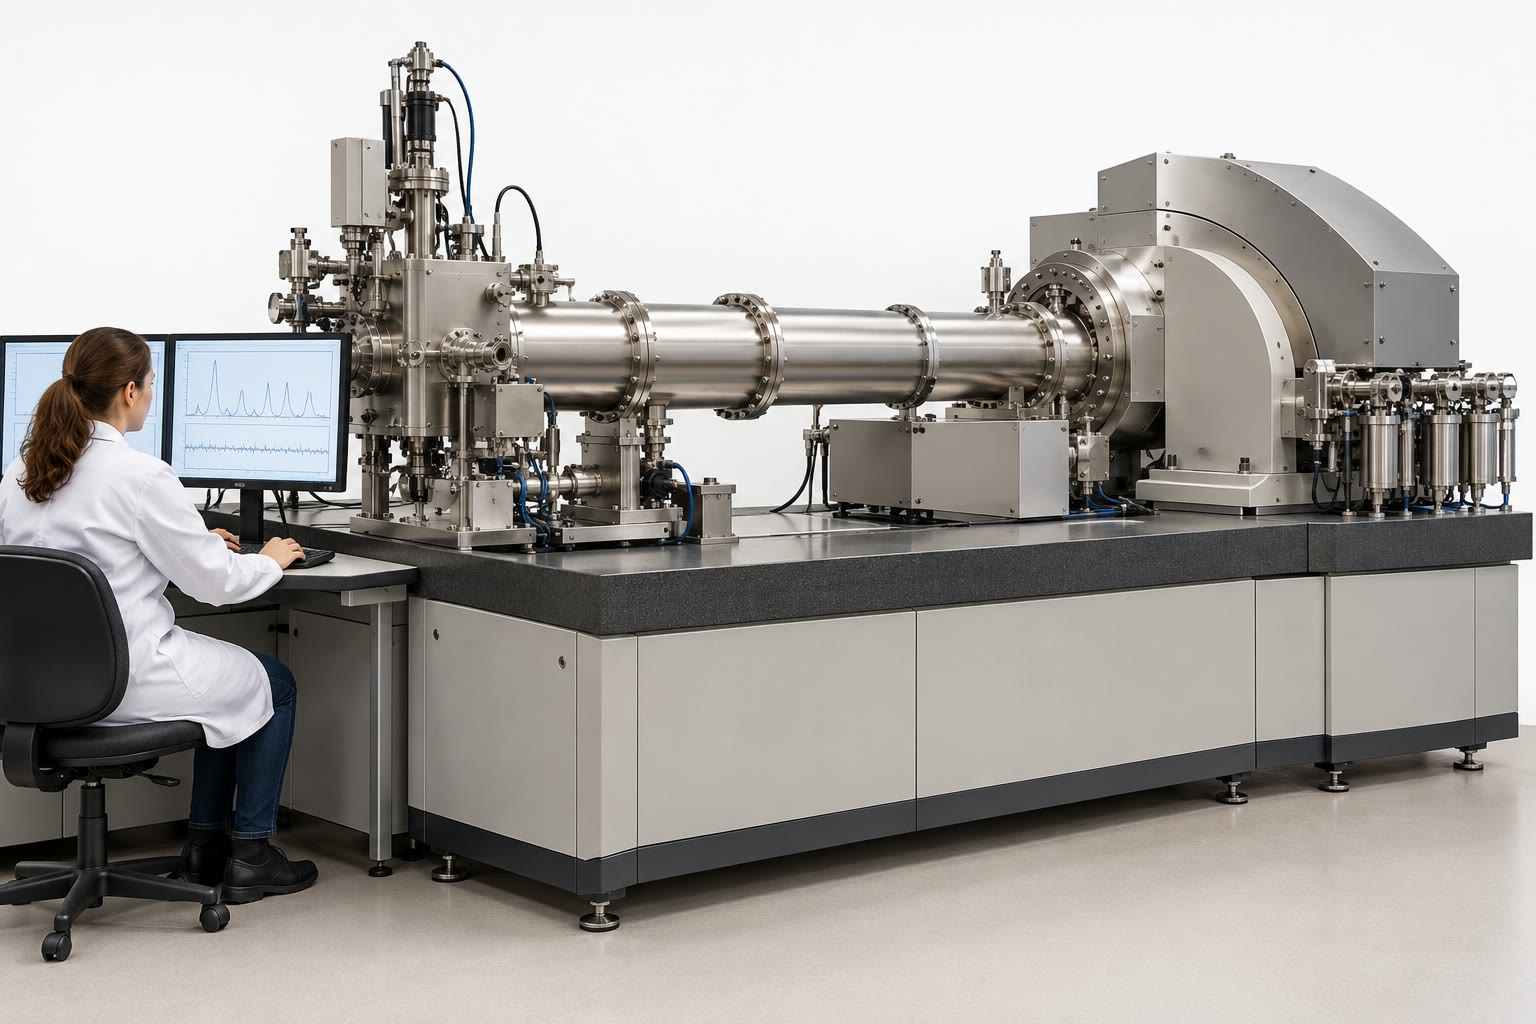
\includegraphics[width=\linewidth]{images/book4/ai/b2-isotope-lab.jpg}
\par\smallskip{\scriptsize Un espectrómetro de masas multicolector en un laboratorio
de isótopos (ilustración generada por IA).}
\end{minipage}
\end{inthelab}
% ledger: white:chur

\section{Ejercicios}

\begin{exercise}[$\star$]\label{exo:b2:isotope-geochemistry:1}
Un basalto de Tristán de Acuña tiene $^{143}\mathrm{Nd}/^{144}\mathrm{Nd} = 0.51249$ y
uno de Mangaia 0.51285. Calcúlense sus $\varepsilon_{\mathrm{Nd}}$ y la del MORB
medio (0.513074). ¿Qué fuentes han tenido una Sm/Nd más alta que las \omterm{def:b2:planet-formation-meteorites:chondrule}{condritas}?
\end{exercise}

\begin{exercise}[$\star$]\label{exo:b2:isotope-geochemistry:2}
La razón $^{18}\mathrm{O}/^{16}\mathrm{O}$ vale \num{2.0052e-3} en el \omterm{def:b2:isotope-geochemistry:standards}{VSMOW} y
\num{2.0672e-3} en el \omterm{def:b2:isotope-geochemistry:standards}{VPDB}. ¿Cuál es el $\delta^{18}\mathrm{O}$ del \omterm{def:b2:isotope-geochemistry:standards}{VPDB} en la escala
\omterm{def:b2:isotope-geochemistry:standards}{VSMOW}? Una calcita tiene $\delta^{18}\mathrm{O} = -2.0$ por mil (\omterm{def:b2:isotope-geochemistry:standards}{VPDB}); calcúlense su razón
y su $\delta^{18}\mathrm{O}$ en la escala \omterm{def:b2:isotope-geochemistry:standards}{VSMOW}.
\end{exercise}

\begin{exercise}[$\star$]\label{exo:b2:isotope-geochemistry:3}
Calcúlese la razón $^{143}\mathrm{Nd}/^{144}\mathrm{Nd}$ del CHUR hace \qty{1.0}{Ga} y
hace \qty{4.567}{Ga} ($\lambda_{147} = \qty{6.524e-12}{\per\year}$,
$^{147}\mathrm{Sm}/^{144}\mathrm{Nd} = 0.1966$, hoy 0.512638).
\end{exercise}

\begin{exercise}[$\star$]\label{exo:b2:isotope-geochemistry:4}
Una muestra de nieve de una estación de montaña tiene $\delta^{18}\mathrm{O} = -18.0$ por mil.
¿Qué $\delta\mathrm{D}$ predice la \omterm{prop:b2:isotope-geochemistry:mwl}{recta de agua meteórica}? Un agua de lago tiene
$\delta^{18}\mathrm{O} = -4.0$ y $\delta\mathrm{D} = -42$ por mil: calcúlese su exceso
de deuterio $d = \delta\mathrm{D} - 8\delta^{18}\mathrm{O}$, y dígase si está por encima o
por debajo de la recta.
\end{exercise}

\begin{exercise}[$\star\star$]\label{exo:b2:isotope-geochemistry:5}
Evalúese el $Q$ de la proposición del crecimiento lineal. Un granito tiene Sm \qty{6.0}{ppm}
y Nd \qty{30}{ppm} (CI: 0.145 y \qty{0.457}{ppm}). Calcúlense su
$f_{\mathrm{Sm/Nd}}$ y el cambio de su $\varepsilon_{\mathrm{Nd}}$ en
\qty{500}{Myr}.
\end{exercise}

\begin{exercise}[$\star\star$]\label{exo:b2:isotope-geochemistry:6}
Una corteza se separó hace \qty{2.7}{Ga} de un manto con
$\varepsilon_{\mathrm{Nd}} = +3.5$, con $f_{\mathrm{Sm/Nd}} = -0.45$. Estímese su
$\varepsilon_{\mathrm{Nd}}$ actual con la proposición del crecimiento lineal. El cálculo
exacto da $-27.3$; ¿en cuánto difiere la aproximación, y por qué es
demasiado alta o demasiado baja?
\end{exercise}

\begin{exercise}[$\star\star$]\label{exo:b2:isotope-geochemistry:7}
Un magma basáltico (Sr \qty{130}{ppm}, $^{87}\mathrm{Sr}/^{86}\mathrm{Sr} = 0.7030$)
asimila un granito (Sr \qty{320}{ppm}, 0.7200). Calcúlese la razón
$^{87}\mathrm{Sr}/^{86}\mathrm{Sr}$ de mezclas con un 5, un 10 y un 20 por ciento de granito.
Demuéstrese que $^{87}\mathrm{Sr}/^{86}\mathrm{Sr}$ es una recta frente a $1/\mathrm{Sr}$
y dense su pendiente y su ordenada en el origen.
\end{exercise}

\begin{exercise}[$\star\star$]\label{exo:b2:isotope-geochemistry:8}
Con los factores de fraccionamiento líquido--vapor 1.0098 ($^{18}$O) y 1.084 (D) a
\qty{20}{\degreeCelsius}, calcúlense el $\delta^{18}\mathrm{O}$ y el $\delta\mathrm{D}$ de un
vapor en equilibrio con el agua oceánica (0, 0), y la pendiente
$\delta\mathrm{D}/\delta^{18}\mathrm{O}$ de la recta que va del agua al vapor. Repítase
a \qty{0}{\degreeCelsius} (1.0117 y 1.111). Compárese con la \omterm{prop:b2:isotope-geochemistry:mwl}{recta de agua meteórica}.
\end{exercise}

\begin{exercise}[$\star\star$]\label{exo:b2:isotope-geochemistry:9}
La corteza continental es el 0.51 por ciento de la masa de la Tierra silicatada y contiene,
de media, \qty{27}{ppm} de Nd frente a \qty{1.25}{ppm} en la Tierra silicatada. Tómese
la $\varepsilon_{\mathrm{Nd}}$ de la corteza como $-15$ y la de la Tierra silicatada como 0. ¿Qué
proporción del neodimio contiene la corteza? Si el resto del manto fuera uniforme,
¿cuál sería su $\varepsilon_{\mathrm{Nd}}$? ¿Qué proporción del neodimio debe contener un
reservorio empobrecido a $+8.5$ si el resto del manto es condrítico?
\end{exercise}

\begin{exercise}[$\star\star\star$]\label{exo:b2:isotope-geochemistry:10}
Demuéstrese que en la proposición del crecimiento lineal los términos despreciados tienen un tamaño
relativo de cerca de $\lambda t/2$. A lo largo de la edad de la Tierra, ¿cuánto vale, y qué
error causa en $\varepsilon_{\mathrm{Nd}}$ para $f = -0.45$ a lo largo de
\qty{2.7}{Ga}?
\end{exercise}

\begin{exercise}[$\star\star\star$]\label{exo:b2:isotope-geochemistry:11}
Dos componentes tienen razones Sr/Nd de 13.3 (A) y 5.0 (B). Con la demostración de la
\omterm{prop:b2:isotope-geochemistry:mixing}{hipérbola de mezcla}, hállese la proporción $s'$ del estroncio procedente de A en una mezcla en la que A
aporta una proporción $s = 0.5$ del neodimio. ¿Para qué valor de $s$ difieren más las dos
proporciones?
\end{exercise}

\begin{exercise}[$\star\star\star$]\label{exo:b2:isotope-geochemistry:12}
Un modelo de cajas da de 2.3 a 2.6 veces el volumen actual de corteza continental,
\qty{7.2e9}{km^3}, generado desde la formación de la Tierra hace \qty{4.5}{Ga}, y de 1.3 a 1.6
veces destruido. Calcúlense los ritmos medios de generación y de destrucción en
\unit{km^3} por año. Compárense con los ritmos actuales en las zonas de subducción,
\qty{2.7}{km^3} al año añadidos y \qty{3.2}{km^3} al año retirados.
\end{exercise}

\section{Problema: tres islas, tres mantos}

\begin{problem}[{Problema de fin de semana --- situar las lavas de tres islas en la
alineación del manto, separar una mezcla de un tercer componente y datar el
sedimento reciclado}]
\label{pb:b2:isotope-geochemistry:1}
Tres islas volcánicas de un océano imaginario, Kora, Vel y Asha, emiten basaltos
con las razones isotópicas siguientes. Una geoquímica modeliza sus fuentes con dos
componentes: un \omterm{def:b2:isotope-geochemistry:reservoirs}{manto empobrecido} como la fuente del MORB (Sr \qty{10}{ppm}, Nd
\qty{0.75}{ppm}, $^{87}\mathrm{Sr}/^{86}\mathrm{Sr} = 0.70282$,
$^{143}\mathrm{Nd}/^{144}\mathrm{Nd} = 0.51307$) y un sedimento antiguo devuelto al
manto por subducción (Sr \qty{200}{ppm}, Nd \qty{40}{ppm}, $0.72000$, $0.51141$;
$^{147}\mathrm{Sm}/^{144}\mathrm{Nd} = 0.110$, $^{87}\mathrm{Rb}/^{86}\mathrm{Sr} = 0.50$).
Kora: $0.70410$, $0.51278$; Vel: $0.70618$, $0.51242$; Asha: $0.70290$, $0.51288$
($^{87}\mathrm{Sr}/^{86}\mathrm{Sr}$, $^{143}\mathrm{Nd}/^{144}\mathrm{Nd}$). CHUR actual:
$^{143}\mathrm{Nd}/^{144}\mathrm{Nd} = 0.512638$, $^{147}\mathrm{Sm}/^{144}\mathrm{Nd} =
0.1966$; $\lambda_{147} = \qty{6.524e-12}{\per\year}$, $\lambda_{87} =
\qty{1.3972e-11}{\per\year}$.

\medskip\noindent\textbf{Parte I --- Situar las islas.}
\begin{enumerate}
\item Calcúlese la $\varepsilon_{\mathrm{Nd}}$ de los dos componentes.
\item Calcúlese la $\varepsilon_{\mathrm{Nd}}$ de las tres islas.
\item Sitúense las cinco composiciones en un diagrama Sr--$\varepsilon_{\mathrm{Nd}}$. ¿Qué
islas están en el lado enriquecido del CHUR?
\item Asha tiene casi la razón del estroncio del \omterm{def:b2:isotope-geochemistry:reservoirs}{manto empobrecido} pero una
$\varepsilon_{\mathrm{Nd}}$ mucho más baja. ¿Dónde se sitúa respecto a la alineación del manto, y a qué
grupo de islas del capítulo se parece?
\item ¿Por qué pueden tomarse las razones isotópicas de las lavas como las de sus fuentes,
aunque las lavas tengan Sm/Nd y Rb/Sr muy distintas de las de sus fuentes?
\item Una lava de Kora con $^{147}\mathrm{Sm}/^{144}\mathrm{Nd} = 0.12$ tiene \qty{1}{Myr}.
¿Cuánto ha crecido su $^{143}\mathrm{Nd}/^{144}\mathrm{Nd}$ desde la erupción, en
unidades épsilon? ¿Importa?
\end{enumerate}

\noindent\textbf{Parte II --- Mezclar los dos componentes.}
\begin{enumerate}[resume]
\item Escríbanse la concentración de Nd y la razón $^{143}\mathrm{Nd}/^{144}\mathrm{Nd}$ de una
mezcla con una fracción másica $f$ de sedimento.
\item Calcúlese la $\varepsilon_{\mathrm{Nd}}$ de mezclas con $f = 0.5$, 1, 2 y 5 por
ciento.
\item Calcúlese la razón $^{87}\mathrm{Sr}/^{86}\mathrm{Sr}$ de las mismas mezclas.
\item Demuéstrese que la razón $^{87}\mathrm{Sr}/^{86}\mathrm{Sr}$ de las mezclas es una recta
frente a $1/\mathrm{Sr}$, y dese su pendiente.
\item Calcúlese $K = (\mathrm{Sr}/\mathrm{Nd})_{\text{manto}}/(\mathrm{Sr}/\mathrm{Nd})_{\text{sedimento}}$.
¿Qué razón, la del Sr o la del Nd, se acerca más deprisa al sedimento al crecer $f$?
\item ¿Cuántas veces es el sedimento más rico que el manto en Nd, y en Sr?
Explíquese con estos números por qué un uno por ciento de sedimento desplaza
$\varepsilon_{\mathrm{Nd}}$ en unas 11 unidades.
\item ¿Qué proporción del neodimio de una mezcla con $f = 1$ por ciento procede del
sedimento?
\end{enumerate}

\noindent\textbf{Parte III --- ¿Cuánto sedimento?}
\begin{enumerate}[resume]
\item Despéjese $f$ de la ecuación de mezcla del Nd, dada la razón $R$ de la mezcla.
\item Calcúlese $f$ para Kora a partir de su neodimio.
\item Calcúlese $f$ para Kora a partir de su estroncio. ¿Coinciden ambos?
\item Calcúlese $f$ para Vel a partir de su neodimio y de su estroncio.
\item Calcúlese $f$ para Asha a partir de su neodimio, y la razón del estroncio que predice
este $f$. Compárese con el valor medido: ¿qué se concluye sobre la fuente
de Asha?
\item Propóngase un tercer componente para Asha, a partir del capítulo, y las
razones padre--hijo que debió de tener.
\end{enumerate}

\noindent\textbf{Parte IV --- La edad del sedimento.}
\begin{enumerate}[resume]
\item El sedimento se subdujo hace \qty{2.0}{Ga} y ha permanecido cerrado desde entonces.
Calcúlense su $^{143}\mathrm{Nd}/^{144}\mathrm{Nd}$, la del CHUR y su
$\varepsilon_{\mathrm{Nd}}$ en ese momento.
\item Rehágase el cálculo con la proposición del crecimiento lineal.
\item Calcúlese la razón $^{87}\mathrm{Sr}/^{86}\mathrm{Sr}$ del sedimento hace \qty{2.0}{Ga}.
\item Hace \qty{2.0}{Ga}, la corteza de la figura de $\varepsilon_{\mathrm{Nd}}$ tenía
$\varepsilon_{\mathrm{Nd}} \approx -4.7$. ¿Es coherente el valor del sedimento en la subducción
con un origen por erosión de una corteza continental tan joven?
\item Dese la fracción másica de sedimento reciclado en la fuente de la isla más
enriquecida, el número clave de este problema.
\end{enumerate}
\end{problem}
% ledger: white:chur, villa20:sm147, villa22:rb87, gale13:isotopes
